\documentclass[a4paper, 12pt]{article}
\usepackage{graphicx} % Required for inserting images
\usepackage{amsmath}
\usepackage{pgfplots}
\usepackage{tabularx}
\usepgfplotslibrary{dateplot}

\newcommand{\templates}{../../template}
\usepackage[a4paper, margin=2.5cm]{geometry}

\usepackage{enumitem}
\setlist[itemize]{noitemsep}
\setlist[enumerate]{noitemsep}

\let\oldpar\paragraph
\renewcommand{\paragraph}[1]{\oldpar{#1\\}\noindent}

% Avoid dots in the table of contents, it mess with the gulpease calculation
\makeatletter
\renewcommand{\@dotsep}{10000} 
\makeatother
\usepackage{graphicx}
\usepackage{hyperref}
\usepackage{makecell}
\usepackage{fancyhdr}

\newcommand{\settitolo}[1]{\newcommand{\titolo}{#1\\}}
\newcommand{\setprogetto}[1]{\newcommand{\progetto}{#1\\}}
\newcommand{\setcommittenti}[1]{\newcommand{\committenti}{#1\\}}
\newcommand{\setredattori}[1]{\newcommand{\redattori}{#1\\}}
\newcommand{\setrevisori}[1]{\newcommand{\revisori}{#1\\}}
\newcommand{\setresponsabili}[1]{\newcommand{\responsabili}{#1\\}}
\newcommand{\setversione}[1]{
	\ifdefined\versione\renewcommand{\versione}{#1\\}
	\else\newcommand{\versione}{#1\\}\fi
}
\newcommand{\setdestuso}[1]{\newcommand{\uso}{#1\\}}
\newcommand{\setdescrizione}[1]{\newcommand{\descrizione}{#1\\}}

\newcommand{\makefrontpage}{
	\begin{titlepage}
		\begin{center}

		
\includegraphics[width=0.4\textwidth]{\templates/4ourSquared_logo}\\

		{\Large 4OURSQUARED}\\[6pt]
		\href{mailto://4oursquared.unipd@gmail.com}{4oursquared.unipd@gmail.com}\\
		
		\ifdefined\progetto
		\vspace{1cm}
		{\Large\progetto}
		{\large\committenti}
		\else\fi
		
		\vspace{1.5cm}
		{\LARGE\titolo}
		
		\vfill
		
		\begin{tabular}{r | l}
		\multicolumn{2}{c}{\textit{Informazioni}}\\
		\hline
		
		\ifdefined\redattori
			\textit{Redattori} &
			\makecell[l]{\redattori}\\
		\else\fi
		\ifdefined\revisori
			\textit{Revisori} &
			\makecell[l]{\revisori}\\
		\else\fi
		\ifdefined\responsabili
			\textit{Responsabili} &
			\makecell[l]{\responsabili}\\
		\else\fi
		
		\ifdefined\versione
			\textit{Versione} & \versione
		\else\fi
		
		\textit{Uso} & \uso
		
		\end{tabular}
		
		\vspace{2cm}
		
		\ifdefined\descrizione
		Descrizione
		\vspace{6pt}
		\hrule
		\descrizione
		\else\fi
		\end{center}
	\end{titlepage}
}
\usepackage{hyperref}
\usepackage{array}
\usepackage{tabularx}
\usepackage{adjustbox}

\newcounter{verscount}
\setcounter{verscount}{0}
\newcommand{\addversione}[5]{
	\ifdefined\setversione
		\setversione{#1}
	\else\fi
	\stepcounter{verscount}
	\expandafter\newcommand%
		\csname ver\theverscount \endcsname{#1&#2&#3&#4&#5}
}

\newcommand{\listversioni}{
	\ifnum\value{verscount}>1
		\csname ver\theverscount \endcsname
		\addtocounter{verscount}{-1}
		\\\hline
		\listversioni
	\else
		\csname ver\theverscount \endcsname\\\hline
	\fi
}

\newcommand{\makeversioni}{
	\begin{center}
		\begin{tabularx}{\textwidth}{|c|c|c|c|X|}
		\hline
		\textbf{Versione} & \textbf{Data} & \textbf{Redattore} & \textbf{Verificatore} & \textbf{Descrizione} \\
		\hline
		\listversioni
		\end{tabularx}
	\end{center}
	\clearpage
}
\graphicspath{ {./immagini/} }

\settitolo{Piano di Qualifica}
\setredattori{Brotto Romina\\ Salami Lorenzo \\ Soldà Matteo}
\setdestuso{esterno}
\setdescrizione{
Questo documento serve a definire le metriche e i criteri di accettazione dei prodotti.
}


\addversione{0.0.0}{18/04/2023}{Salami Lorenzo}{Soldà Matteo}{Stesura iniziale.}
\addversione{0.0.1}{24/04/2023}{Soldà Matteo}{Salami Lorenzo}{Aggiunta delle intestazioni e dei piè di pagina}
\addversione{0.0.2}{24/07/2023}{Brotto Romina}{Ceccato Francesco}{Aggiunta sezione 3 ed indici}
\addversione{0.1.0}{25/07/2023}{Brotto Romina}{Salami Lorenzo}{Verifica per RTB}
\addversione{1.0.0}{25/07/2023}{Salami Lorenzo}{Brotto Romina}{Versione finale	per RTB}
\addversione{1.0.1}{19/09/2023}{Brotto Romina}{Salami Lorenzo}{Aggiunta sezione di test client}
\addversione{1.0.2}{25/09/2023}{Brotto Romina}{Soldà Matteo}{Aggiunti test server}
\addversione{1.0.3}{26/09/2023}{Brotto Romina}{Soldà Matteo}{Aggiunta sezione code coverage}
\addversione{1.1.0}{26/09/2023}{Alberti Nicolas}{Soldà Matteo}{Verifica per \textit{PB}}
\addversione{2.0.0}{26/09/2023}{Soldà Matteo}{Alberti Nicolas}{Approvazione per candidatura \textit{PB}}


\begin{document}

\makefrontpage
\makeindexdetails
\makeversioni
\tableofcontents
\clearpage
\makecontentsdetails

\section{Qualità di prodotto}

\subsection{Documentazione}
\subsubsection{Indice di Gulpease}
\[ \text{Indice di Gulpease} = 89 + \frac{300*\text{\#frasi} - 10*\text{\#lettere}}{\text{\#parole}} \]
\begin{itemize}
	\item \#lettere: numero di caratteri alfanumerici;
	\item \#parole: numero di gruppi di caratteri alfanumerici;
	\item \#frasi: numero di gruppi di punti o punti e virgola consecutivi.
\end{itemize}

\subparagraph{Prodotti coinvolti:}
\begin{center}
	\begin{tabularx}{\textwidth}{|X|X|X|}
		\hline
		\textbf{Prodotto} & \textbf{Valore accettabile} & \textbf{Valore ottimale } \\
		\hline
		Documenti interni & $>$ 40                      & $>$ 60                    \\
		\hline
		Documenti esterni & $>$ 50                      & $>$ 60                    \\
		\hline
	\end{tabularx}\\[8pt]
	\mbox{}\\
\end{center}

\subparagraph{Riferimenti:} \underline{\href{http://www.corrige.it/leggibilita/lindice-gulpease/}{http://www.corrige.it/leggibilita/lindice-gulpease/}}

\subsection{Prodotti software}

\subsubsection{Copertura statement}
La metrica si basa sullo statement coverage.

\subparagraph{Prodotti coinvolti:}
\begin{center}
	\begin{tabularx}{\textwidth}{|X|X|X|}
		\hline
		\textbf{Prodotto} & \textbf{Valore accettabile } & \textbf{Valore ottimale } \\
		\hline
		Software          & $>$ 70\%                     & $>$ 95\%                  \\
		\hline
	\end{tabularx}\\[8pt]
	\mbox{}\\
\end{center}
\subsubsection{Copertura branch}
La metrica si basa sul branch coverage.

\subparagraph{Prodotti coinvolti:}
\begin{center}
	\begin{tabularx}{\textwidth}{|X|X|X|}
		\hline
		\textbf{Prodotto} & \textbf{Valore accettabile } & \textbf{Valore ottimale } \\
		\hline
		Software          & $>$ 70\%                     & $>$ 80\%                  \\
		\hline
	\end{tabularx}\\[8pt]
	\mbox{}\\
\end{center}

\newpage
\section{Qualità di processo}
\subsubsection{Time variance}
La metrica si basa sulla variazione percentuale rispetto alla stima iniziale.

\subparagraph{Prodotti coinvolti:}
\begin{center}
	\begin{tabularx}{\textwidth}{|X|X|X|}
		\hline
		\textbf{Prodotto} & \textbf{Valore accettabile } & \textbf{Valore ottimale } \\
		\hline
		Software          & $<$ 20\%                     & 0\%                       \\
		\hline
		Documentazione    & $<$ 20\%                     & 0\%                       \\
		\hline
	\end{tabularx}\\[8pt]
	\mbox{}\\
\end{center}
\subsubsection{Budget variance}
La metrica si basa sulla variazione percentuale rispetto alla stima iniziale.

\subparagraph{Prodotti coinvolti:}
\begin{center}
	\begin{tabularx}{\textwidth}{|X|X|X|}
		\hline
		\textbf{Prodotto} & \textbf{Valore accettabile } & \textbf{Valore ottimale } \\
		\hline
		Software          & $<$ 20\%                     & 0\%                       \\
		\hline
		Documentazione    & $<$ 20\%                     & 0\%                       \\
		\hline
	\end{tabularx}\\[8pt]
	\mbox{}\\
\end{center}

\section {Applicazione e valutazione delle metriche}
I grafici sono frutto di un foglio di calcolo creato dal gruppo che applica le formule per il calcolo delle metriche definite in questo documento.
\subsection{Valutazione d’insieme (Qualità di processo)}
L'avanzamento del lavoro è proseguito secondo le aspettative.
È stato riscontrato una diminuzione delle ore lavorate negli sprint 8 e 9 dovuti
a impegni universitari quali esami e consegne.
Questo calo ha particolarmente
influenzato il grafico dello schedule variance che è effettivamente sceso sotto la soglia di tolleranza prefissata dal gruppo.
Lo stesso si può riscontrare nella distanza tra il planned e l’earned value, che
è cresciuta particolarmente durante quegli sprint.

Il gruppo aveva tenuto in considerazione che ci sarebbe stato un calo di lavoro durante gli sprint sopra indicati, prevedendo però di rientrare nei valori di tolleranza negli sprint successivi.



\section{Attività di Testing}
I seguenti test sono stati elencati seguendo l'ordine alfabetico dei nomi dei file in cui si trovano.
\subsection*{Test Client}
\setlength\tabcolsep{4pt}
\begin{center}
	\begin{tabularx}{\textwidth}{|X|X|X|}
		\hline
		\multicolumn{3}{| c |}{\textbf{AreaSingleView.test.tsx file}}                                                       \\
		\hline
		TC4  & Verifica che il fetch delle informazioni riguardanti tutte le aree illuminate avvenga correttamente & RF7-O  \\
		\hline
		TC5  & Verifica che, dopo la cancellazione del lampione, esso sia effettvamente scomparso dalla lista      & RF20-O \\
		\hline
		TC6  & Verifica che, dopo la cancellazione del sensore, esso sia effettvamente scomparso dalla lista       & RF18-O \\
		\hline
		\multicolumn{3}{| c |}{\textbf{AreaTable.test.tsx file}}                                                            \\
		\hline
		TC7  & Verifica che il fetch delle informazioni per la singola area avvenga correttamente                  & RF10-O \\
		\hline
		TC8  & Verifica che la riconfigurazione dell'area illuminata avvenga con successo                          & RF11-O \\
		\hline
		TC9  & Verifica che la rimozione dell'area illuminata avvenga con successo                                 & RF12-O \\
		\hline
		TC10 & Verifica che la rimozione dell'area illuminata venga annullata senza modificarne il contenuto       & Rf12-O \\
		\hline
		\multicolumn{3}{| c |}{\textbf{Content.test.tsx file}}                                                              \\
		\hline
		TC11 & Verifica che la pagina di elenco aree illuminate si carichi correttamente (anche se vuota)          & RF7-O  \\
		\hline
		\multicolumn{3}{| c |}{\textbf{EditAreaForm.test.tsx file}}                                                         \\
		\hline
		TC12 & Verifica che il form di modifica area illuminata venga visualizzato correttamente                   & RF11-O \\
		\hline
		\multicolumn{3}{| c |}{\textbf{EditLampForm.test.tsx file}}                                                         \\
		\hline
		TC13 & Verifica che il form di modifica lampione venga visualizzato correttamente                          & RF11-O \\
		\hline
		\multicolumn{3}{| c |}{\textbf{EditSensorForm.test.tsx file}}                                                       \\
		\hline
		TC14 & Verifica che il form di modifica sensore venga visualizzato correttamente                           & RF39-O \\
		\hline
	\end{tabularx}\\[8pt]
	\mbox{}\\
\end{center}



\begin{center}
	\begin{tabularx}{\textwidth}{|X|X|X|}
		\hline
		\textbf{Codice} & \textbf{Descrizione }                                                                                                            & \textbf{Requisiti collegati } \\
		\hline
		\multicolumn{3}{| c |}{\textbf{Footer.test.tsx file}}                                                                                                                              \\
		\hline
		TC15            & Verifica che il footer comune a tutte le pagine venga visualizzato correttamente                                                 & -                             \\
		\hline
		\multicolumn{3}{| c |}{\textbf{Header.test.tsx file}}                                                                                                                              \\
		\hline
		TC16            & Verifica che il render del modulo header per il logout e il footer avvengano correttamente                                       & -                             \\
		\hline
		\multicolumn{3}{| c |}{\textbf{LampCard.test.tsx file}}                                                                                                                            \\
		\hline
		TC17            & Verifica che il render della scheda dettagli lampione sia visualizzata correttamente                                             & RF19-O                        \\
		\hline
		\multicolumn{3}{| c |}{\textbf{LampGuastiPage.test.tsx file}}                                                                                                                      \\
		\hline
		T18             & Verifica che il render della pagina dedicata all'elenco aree illuminate segnalate guaste avvenga correttamente                   & RF8-O, RV2-O                  \\
		\hline
		\multicolumn{3}{| c |}{\textbf{LampGuastiTable.test.tsx file}}                                                                                                                     \\
		\hline
		TC19            & Verifica che il load della tabella per l'elenco delle aree illuminate segnalate guaste avvenga correttamente                     & RF8-O, RV2-O                  \\
		\hline
		TC20            & Verifica che la rimozione dell'area illuminata dall'elenco delle aree guaste avvenga con successo                                & RF16-O                        \\
		\hline
		TC21            & Verifica che la rimozione dell'area illuminata dall'elenco delle aree guaste venga annullata                                     & RF12-O                        \\
		\hline
		\multicolumn{3}{| c |}{\textbf{LampSingleView.test.tsx file}}                                                                                                                      \\
		\hline
		TC22            & Verifica che il caricamento dei dati relativi al lampione avvenga correttamente                                                  & RF11-O                        \\
		\hline
		TC23            & Verifica che il caricamento dei dati relativi alla tabella dettagli lampione avvenga correttamente                               & RF11-O                        \\
		\hline
		TC24            & Verifica che l'annullamento dell'eliminazione avvenga correttamente                                                              & RF20-O                        \\
		\hline
		TC25            & Verifica che l'annullamento della segnalazione di un lampione guasto avvenga correttamente                                       & RF9-O                         \\
		\hline
		\multicolumn{3}{| c |}{\textbf{LampTableManutentore.test.tsx file}}                                                                                                                \\
		\hline
		TC26            & Verifica che il caricamento dei dati relativi alle aree guaste avvenga correttamente                                             & RF8-O, RV2-O                  \\
		\hline
		\multicolumn{3}{| c |}{\textbf{LoginPage.test.tsx file}}                                                                                                                           \\
		\hline
		TC27            & Verifica che il client renderizzi correttamete la pagina di login.                                                               & RF5-O, RV1-O                  \\
		\hline
		TC28            & Verifica che le credenziali inserite siano corrette e che al click del pulsante "Entra" il login abbia successo                  & RF5-O, RV1-O                  \\
		\hline
		TC29            & Verifica che le credenziali inserite non siano corrette e che al click del pulsante "Entra" il login \textit{non} abbia successo & RF5-O, RV1-O                  \\
		\hline
		\multicolumn{3}{| c |}{\textbf{NewAreaForm.test.tsx file}}                                                                                                                         \\
		\hline
		TC30            & Verifica che il caricamento del form di aggiunta nuova area illuminata avvenga correttamente                                     & RF10-O                        \\
		\hline
		\multicolumn{3}{| c |}{\textbf{NewAreaPage.test.tsx file}}                                                                                                                         \\
		\hline
		Tc31            & Verifica che il caricamento della pagina per l'aggiunta nuova area illuminata avvenga correttamente                              & RF10-O                        \\
		\hline
		\multicolumn{3}{| c |}{\textbf{NewLampForm.test.tsx file}}                                                                                                                         \\
		\hline
		TC32            & Verifica che il caricamento del form di aggiunta nuovo lampione illuminata avvenga correttamente                                 & RF19-O                        \\
		\hline
		\multicolumn{3}{| c |}{\textbf{NewLampPage.test.tsx file}}                                                                                                                         \\
		\hline
		TC33            & Verifica che il caricamento della pagina per l'aggiunta di un lampione avvenga correttamente                                     & RF19-O                        \\
		\hline
		\multicolumn{3}{| c |}{\textbf{NewSensPage.test.tsx file}}                                                                                                                         \\
		\hline
		TC34            & Verifica che il caricamento della pagina per l'aggiunta di un sensore avvenga correttamente                                      & RF17-O                        \\
		\hline
	\end{tabularx}\\[8pt]
	\mbox{}\\
\end{center}



\begin{center}
	\begin{tabularx}{\textwidth}{|X|X|X|}
		\hline
		\textbf{Codice} & \textbf{Descrizione }                                                                                                 & \textbf{Requisiti collegati } \\
		\hline
		\multicolumn{3}{| c |}{\textbf{NewSensorForm.test.tsx file}}                                                                                                            \\
		\hline
		TC35            & Verifica che il caricamento delform per l'aggiunta di un sensore avvenga correttamente                                & RF17-O                        \\
		\hline
		\multicolumn{3}{| c |}{\textbf{PageFullView.test.tsx file}}                                                                                                             \\
		\hline
		TC36            & Verifica se sono presenti header, main e footer in tutte le pagine                                                    & -                             \\
		\hline
		\multicolumn{3}{| c |}{\textbf{SensorSingleView.test.tsx file}}                                                                                                         \\
		\hline
		TC37            & Verifica che il caricamento dei dati relativi al sensore avvenga correttamente                                        & RF39-O                        \\
		\hline
		TC38            & Verifica che il sensore invii correttamente il segnale per scatenare la modifica dell'intensità luminosa del lampione & RF27-O,RF14-O                 \\
		\hline
	\end{tabularx}\\[8pt]
	\mbox{}\\
\end{center}

\subsection*{Test Server}
\setlength\tabcolsep{4pt}
\begin{center}
	\begin{tabularx}{\textwidth}{|X|X|}
		\hline
		\textbf{Codice} & \textbf{Descrizione }                                                                                                                                                                                                                                                                                \\
		\hline
		\multicolumn{2}{| c |}{\textbf{AccountRoutes.test.ts file}}                                                                                                                                                                                                                                                            \\
		\hline
		TS1             & Verifica che il meccanismo di login funzioni correttamente: ritorna 401 se l'username non è presente, 401 se la password è errata.                                                                                                                                                                   \\
		\hline
		TS2             & Verifica che il meccanismo di logout funzioni correttamente: ritorna 403 se non è stato passato un token valido, ritorna 200 se è stato passato un token valido.                                                                                                                                     \\
		\hline
		TS3             & Verifica che la registrazione di un nuovo utente avvenga correttamente: ritorna 200 e crea un nuovo utente con successo, ritorna errore 409 se l'username esiste già, ritorna errore 409 se la mail esiste già.                                                                                      \\
		\hline
		TS4             & Verifica sl passaggio dei token: ritorna 403 se non è stato passato un token valido, ritorna 200 se è stato passato un token valido.                                                                                                                                                                 \\
		\hline
		TS5             & Verifica il recupero della lista utenti: lista completa e/o utente specifico se l'utente è admin, ritorna 500 se l'utente non è autorizzato.                                                                                                                                                         \\
		\hline
		TS6             & Verifica che l'aggiornamento dati utente avvenga correttamente: ritorna 404 se l'utente non è presente, 200 se l'utente è stato aggiornato.                                                                                                                                                          \\
		\hline
		\multicolumn{2}{| c |}{\textbf{AreaRoutes.test.ts file}}                                                                                                                                                                                                                                                               \\
		\hline
		TS7             & Verifica che i dati dell'area illuminata vengano ricevuti correttamente in modalità GET: ritorna 500 se non è possibile recuperare le aree, ritorna 200 e l'area in base all'id fornito, ritorna 404 se l'area non è presente, 500 se non è possibile recuperare l'area specificata dall'id fornito. \\
		\hline
		TS8             & Verifica il funzionamento della creazione di un'area illuminata in modalità POST: ritorna 200 se l'area viene creata correttamente, 500 altrimenti.                                                                                                                                                  \\
		\hline
		TS9             & Verifica che l'aggiornamento di un'area in modalità PUT avvenga correttamente: ritorna 200 se l'area viene aggiornata correttamente, 404 se l'area non viene trovata, 500 se l'area non viene aggiornata correttamente.                                                                              \\
		\hline
	\end{tabularx}\\[8pt]
	\mbox{}\\
\end{center}

\begin{center}
	\begin{tabularx}{\textwidth}{|X|X|}
		\hline
		TS10 & Verifica l'eliminazione di un'area: ritorna 200 se l'area viene eliminata correttamente, 404 l'area da eliminare non viene trovata, 500 se avviene un errore.                                                                                                 \\
		\hline
		\multicolumn{2}{| c |}{\textbf{LampRoutes.test.ts file}}                                                                                                                                                                                                             \\
		\hline
		TS11 & Verifica del recupero delle info del singolo lampione in modalità GET: ritorna 200 nel recupero del singolo lampione, 404 nel recupero di un lampione non esistente e di un lampione di un'area non esistente, 500 nel caso di un errore durante il recupero. \\
		\hline
		TS12 & Verifica del recupero delle info di tutti i lampioni in modalità GET: ritorna 200 se recupera correttamente tutti i lampioni,  404 se non viene trovata l'area di riferimento, 500 se avviene un errore durante il recupero.                                  \\
		\hline
		TS13 & Verifica per l'inserimento di un lampione in modalità POST: ritorna 200 se il lampione viene aggiunto, 500 in caso di errore durante l'inserimento.                                                                                                           \\
		\hline
		TS14 & Verifica per la modifica di un lampione in modalità PUT: ritorna 200 se il lampione non guasto viene segnalato come guasto, 404 se non è presente il lampione o se non esiste l'area, 500 se avviene un errore durante la modifica.                           \\
		\hline
		TS15 & Verifica per la richiesta di supporto alla modifica della luminosità dei lampioni: ritorna 200 se la richiesta di supporto è stata effettuata correttamente, 404 se non è presente l'area, 500 se avviene un errore.                                          \\
		\hline
		TS16 & Verifica per la cancellazione di un lampione: ritorna 200 se il lampione viene cancellato, 404 se non è presente l'area con il lampione da rimuovere,  500 in caso di errore.                                                                                 \\
		\hline
		TS17 & Verifica per i lampioni guasti con utente manutentore: ritorna 200 se il lampione viene tolto dai guasti, 409 se il lampione non è presente, 500 se avviene un errore.                                                                                        \\
		\hline
		TS18 & Verifica per  il recupero dei lampioni guasti: ritorna  200 se recupera correttamente tutti i lampioni guasti, 404 se non viene trovata l'area specificata.                                                                                                   \\
		\hline
	\end{tabularx}\\
	\mbox{}\\
\end{center}


\begin{center}
	\begin{tabularx}{\textwidth}{|X|X|}
		\hline
		\multicolumn{2}{| c |}{\textbf{SensorRoutes.test.ts file}}                                                                                                                                                                                                                 \\
		\hline
		TS19 & Verifica del recupero delle informazioni dei sensori in modalità GET: se l'area esiste ritorna 200 e la lista di tutti i sensori presenti, ritorna 404 se l'area non esiste, 500 se non è possibile recuperare l'area specificata dall'id.                          \\
		\hline
		TS20 & Verifica del recupero delle info del singolo sensore in modalità GET: ritorna 200 se area e sensore richiesti esistono, 404 se l'area esiste ma non il sensore o l'area non esiste                                                                                  \\
		\hline
		TS21 & Verifica per l'inserimento di un sensore in modalità POST: ritorna 200 se l'area esiste,  400 se l'area non esiste, 500 se avviene un errore nel processo di creazione del sensore.                                                                                 \\
		\hline
		TS22 & Verifica per la modifica di un sensore in modalità PUT: ritorna 200 se il sensore che si cerca di modificare esiste, 404 se non esiste                                                                                                                              \\
		\hline
		TS23 & Verifica per la cancellazione di un sensore: ritorna 200 se il sensore che si cerca di eliminare esiste, 404 se il sensore appartiene a un'area inesistente, 500 per un errore durante il processo.                                                                 \\
		\hline
		\multicolumn{2}{| c |}{\textbf{SignalRoutes.test.ts file}}                                                                                                                                                                                                                 \\
		\hline
		TS24 & Verifica funzionamento accensione e spegnimento in modalità PUSH: ritorna 400 se l'area non è stata trovata, ritorna 200 se esiste l'area e i lampioni vengono accesi, 500 in caso di errore                                                                        \\
		\hline
		TS25 & Verifica il post di un segnale: ritorna 200 ed aggiunge il segnale                                                                                                                                                                                                  \\
		\hline
		TS26 & Verifica la generazione di un token: ritorna 200 se il token viene generato correttamente.                                                                                                                                                                          \\
		\hline
		TS27 & Verifica di un token: ritorna 226 se il token è stato utilizzato, 218 se il token è valido e non è stato utilizzato, 200 se il token è valido ed è stato usato ma vanno spenti i lampioni, 498 se il token non è stato trovato,  400 se l'area non è stata trovata. \\
		\hline
	\end{tabularx}\\
	\mbox{}\\
\end{center}
\newpage
\section{Code Coverage}
Dopo aver consultato il committente, siamo giunti alla conclusione che la
percentuale di code coverage desiderabile poteva essere abbassata dall'80'\%
iniziale al 70\%. Il motivo di questa scelta risiede nel fatto che il codice
testato è molto modulare e dipende da librerie esterne non controllate
direttamente dal gruppo, quindi di conseguenza da non considerare durante l'attività di Testing.

Di seguito riportiamo le \textit{Code Coverage} per il client ed il server.

\subsection*{Client Code Coverage}
\begin{center}
	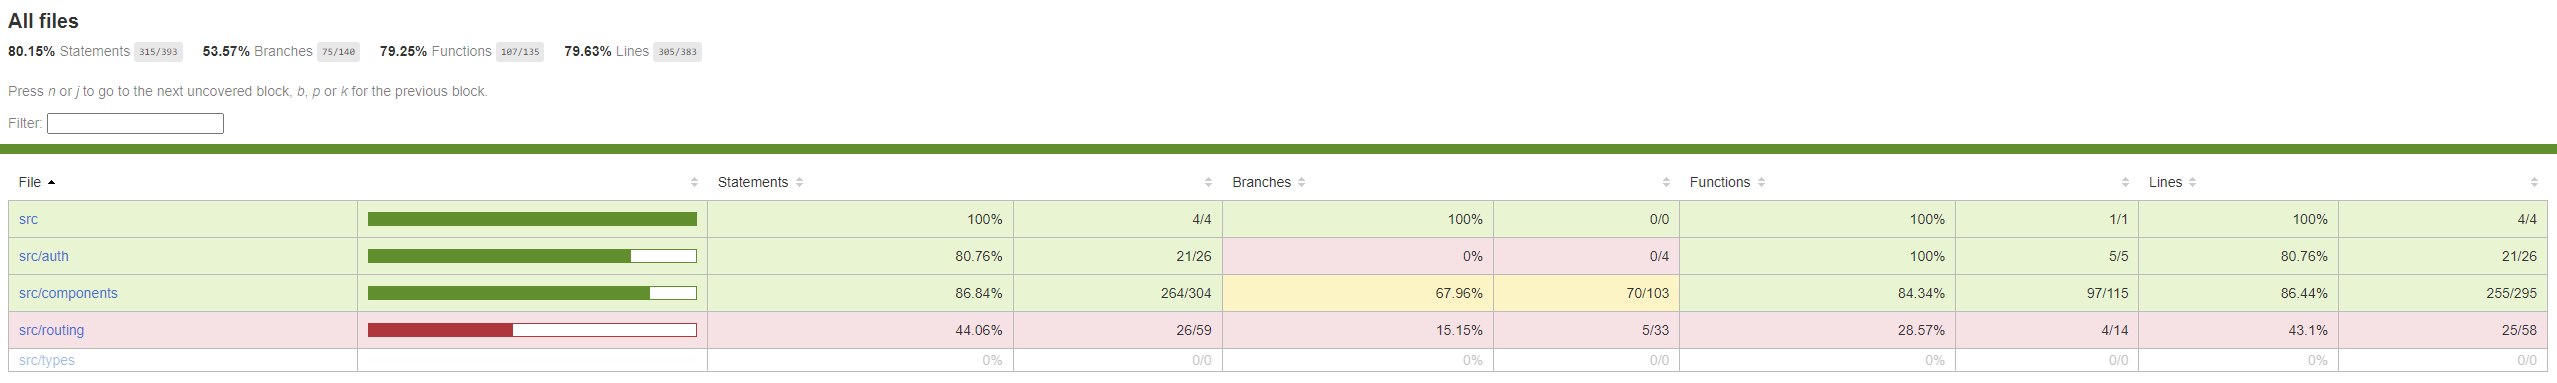
\includegraphics[scale=0.20]{client-coverage.png}
\end{center}
\subsection*{Server Code Coverage}
\begin{center}
	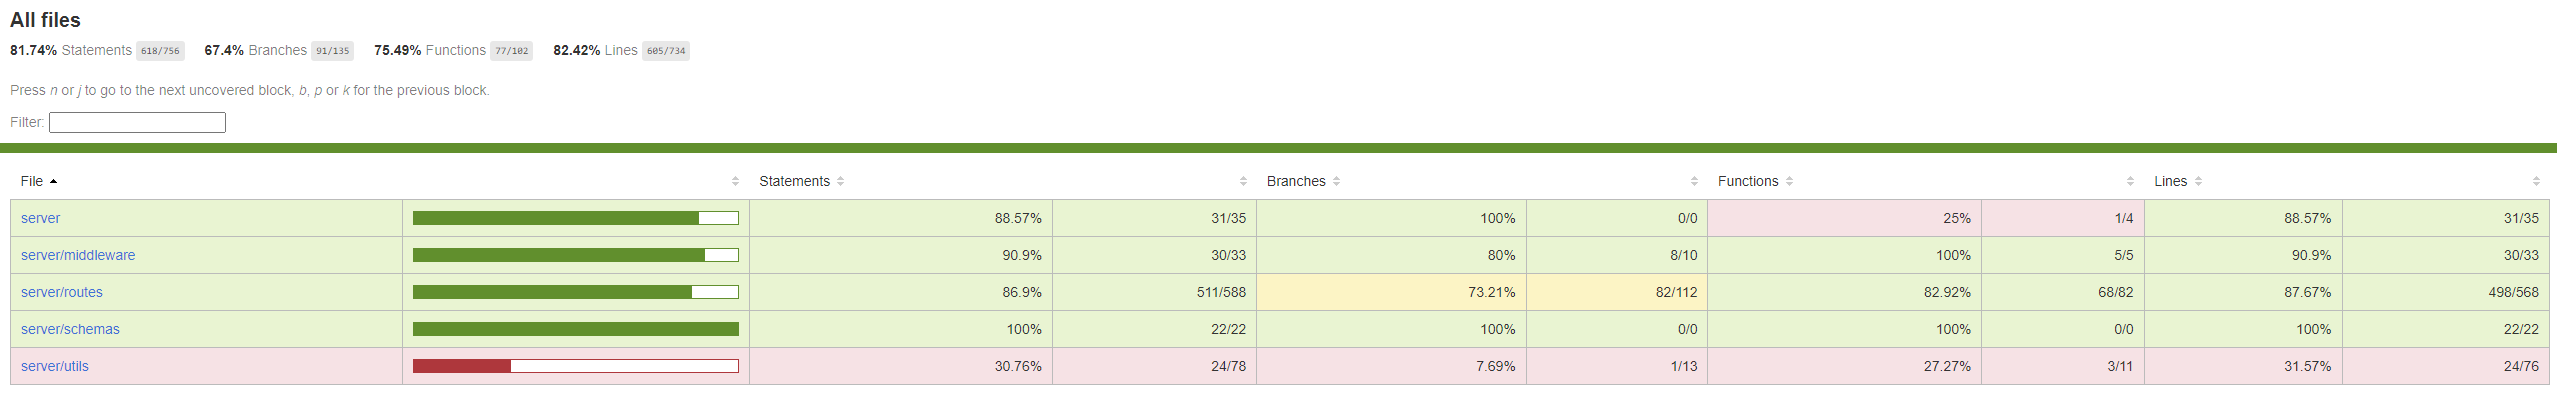
\includegraphics[scale=0.20]{server-coverage.png}
\end{center}

\section{Metriche}
\subsection*{Planning Value, Actual Cost e Earned Value}
\begin{center}
	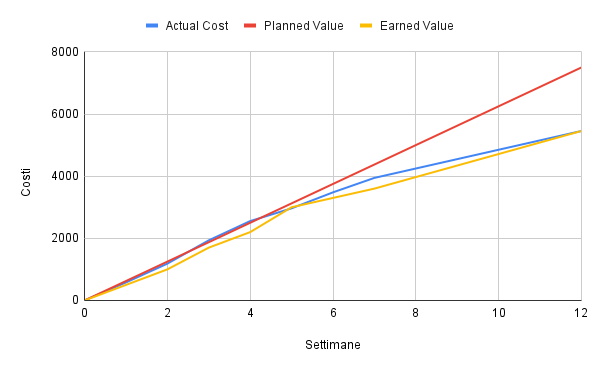
\includegraphics[scale=0.5]{AC_PV_EV.png}
\end{center}


\subsection*{Cost Variance e Schedule Variance}
\begin{center}
	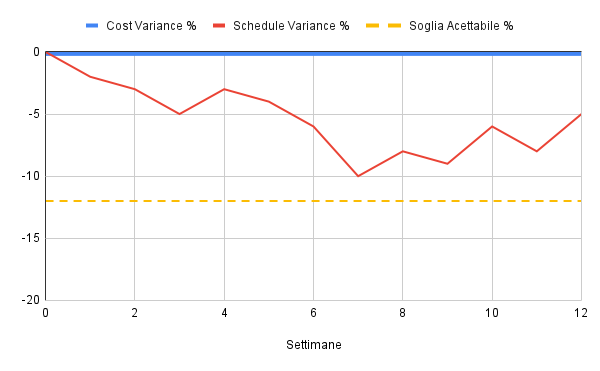
\includegraphics[scale=0.5]{Cost_Variance_Schedule_Variance.png}
\end{center}

\subsection*{Eastimate at completition e Estimate to Complete}
\begin{center}
	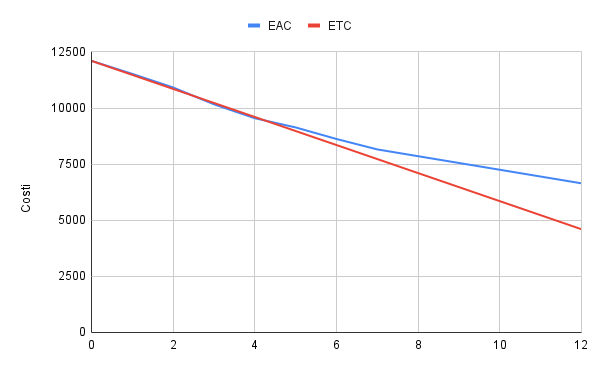
\includegraphics[scale=0.6]{EAC_ETC.png}
\end{center}
\subsection{Cost Performance Index}
\begin{center}
	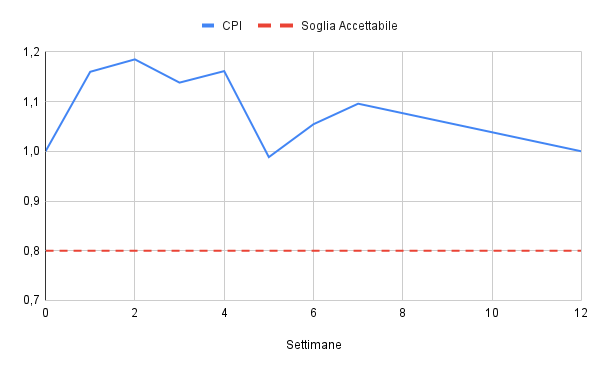
\includegraphics[scale=0.6]{CPI.png}
\end{center}

\subsection*{Indice di Gulpease}
I valori riportati sono frutto di un'analisi approssimativa, usando la libreria PyPdf2 per Python 3.
\begin{center}
	\begin{tabularx}{\textwidth}{|X|X|X|X|X|}
		\hline
		\textbf{Documento}    & \textbf{Frasi } & \textbf{Parole } & \textbf{Caratteri } & \textbf{Indice } \\
		\hline
		Analisi dei requisiti & 839             & 5642             & 34407               & 73               \\
		\hline
		Piano di Progetto     & 253             & 1317             & 7273                & 91               \\
		\hline
		Piano di Qualifica    & 43              & 179              & 1128                & 98               \\
		\hline
		Norme di Progetto     & 423             & 3228             & 17766               & 73               \\
		\hline
		Glossario             & 131             & 984              & 5096                & 77               \\
		\hline
	\end{tabularx}\\[8pt]
	\mbox{}\\
\end{center}

\end{document}